\chapter{Related Work}\label{chapter:relatedwork}

In cyber security community, there are already existing platforms to gain practical experience over browser. "Hack the box", is one of the well-known cyber security education platform however both working principle and its skeleton is different. It is commercial market player rather than non-profit organization, which brings some barriers to some people. 
It has both VPN and virtual machine on browser feature, yet, it is limited with two hours in free plan.


\begin{figure}[htbp]
\centerline{
\includegraphics[scale=.7]{figures/hack-the-box-pricing.png}}
\caption{Taken from https://www.hackthebox.com/hacker/pricing}
\label{fig}
\end{figure}
 

"Hack The Box" platform is great, extensive and well-known, but, it expanded in all kinds of fields from business to certification programs. It makes difficult for the people who want to have easy start with simple approach. Although the platform itself has great resources, user interface, it lacks from simplicity. Here, the target group of "Hack The Box" differs, the argument can be discussed from variety of angle.

Another platform called "TryHackMe", it also contains all different challenges, exercises and virtual machine on browser, enables participants to install nothing on their computer. Similarly, "Hack The Box" platform it has commercial purposes which is absolutely fair. However, considering some beginners who has no information about installing virtual private network to a computer, they might need a subscription. 

\begin{figure}[htbp]
\centerline{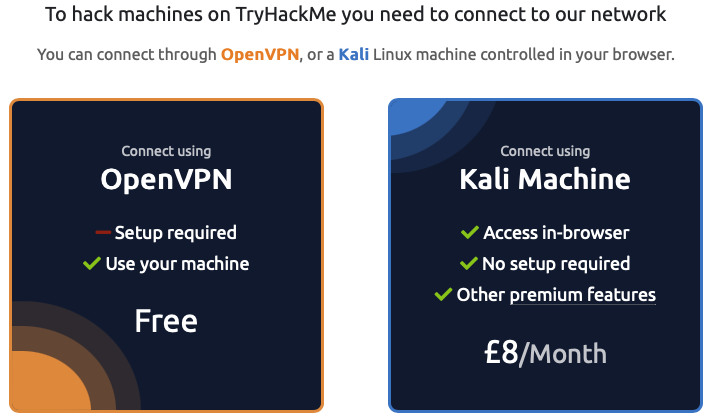
\includegraphics[scale=.5]{figures/try-hack-me.png}}
\caption{Taken from https://tryhackme.com/access}
\label{fig}
\end{figure}
 
 
Even though they are affordable at some extent, the main problem comes when customized, curricula based exercises are required by universities. Furthermore, there is no full control of platform by universities in any of mentioned platforms, except Haaukins. 

Another platform which is also developed by a university is PicoCTF\cite{183443}.
It provides variety of challenges in different categories in a game based environment. It is mostly competition based platform where users has profiles and gain points in time. The points are permanent in the system and can be build on top of them. It is opposite of what Haaukins platform is providing.
Although existing platforms are providing decent environments for cyber security practices, they have different target groups, approaches and policies in terms of their usage. Additionally, the requirements of an exercise in a lecture varies, ideally, the exercise should not be publicly available to prevent cheating. It is hard to achieve for any e-Learning platforms in particular when it is mostly practical exercises. Most of the solutions to exercises on well-known platforms are exists on the internet. Last but not least, Haaukins platform is non-profit platform which allows participants to have fun for free. 